\chapter{Architektur}
\label{cha:Architektur}

\section{Statische Architektur}
% mit Component diagramm
Wie in Kapitel~\ref{cha:Einführung} bereits erwähnt, wird das System BlindControl in drei Komponenten unterteilt. Abbildung~\ref{fig:component_diagramm} stellt den Aufbau des Systems in Form eines Component Diagramm dar. Das ''Sensor Modul'' misst die aktuelle Helligkeit, sowie die Windstärke und überträgt diese auf dem entsprechenden MQTT Topic. Von dort kann der ''Regler'' die aktuellen Sensordaten auslesen und mit dem ihm vermittelten Sollwerten vergleichen. Wird eine neue Position angefahren, gibt der Regler den neuen Beschattungsstand mit Hilfe einer MQTT Nachricht an das ''Aktor Modul'' weiter. Dieses wiederum steuert entsprechend dieser Nachricht die Jalousie an.
\begin{figure}[hbt]
	\centering
	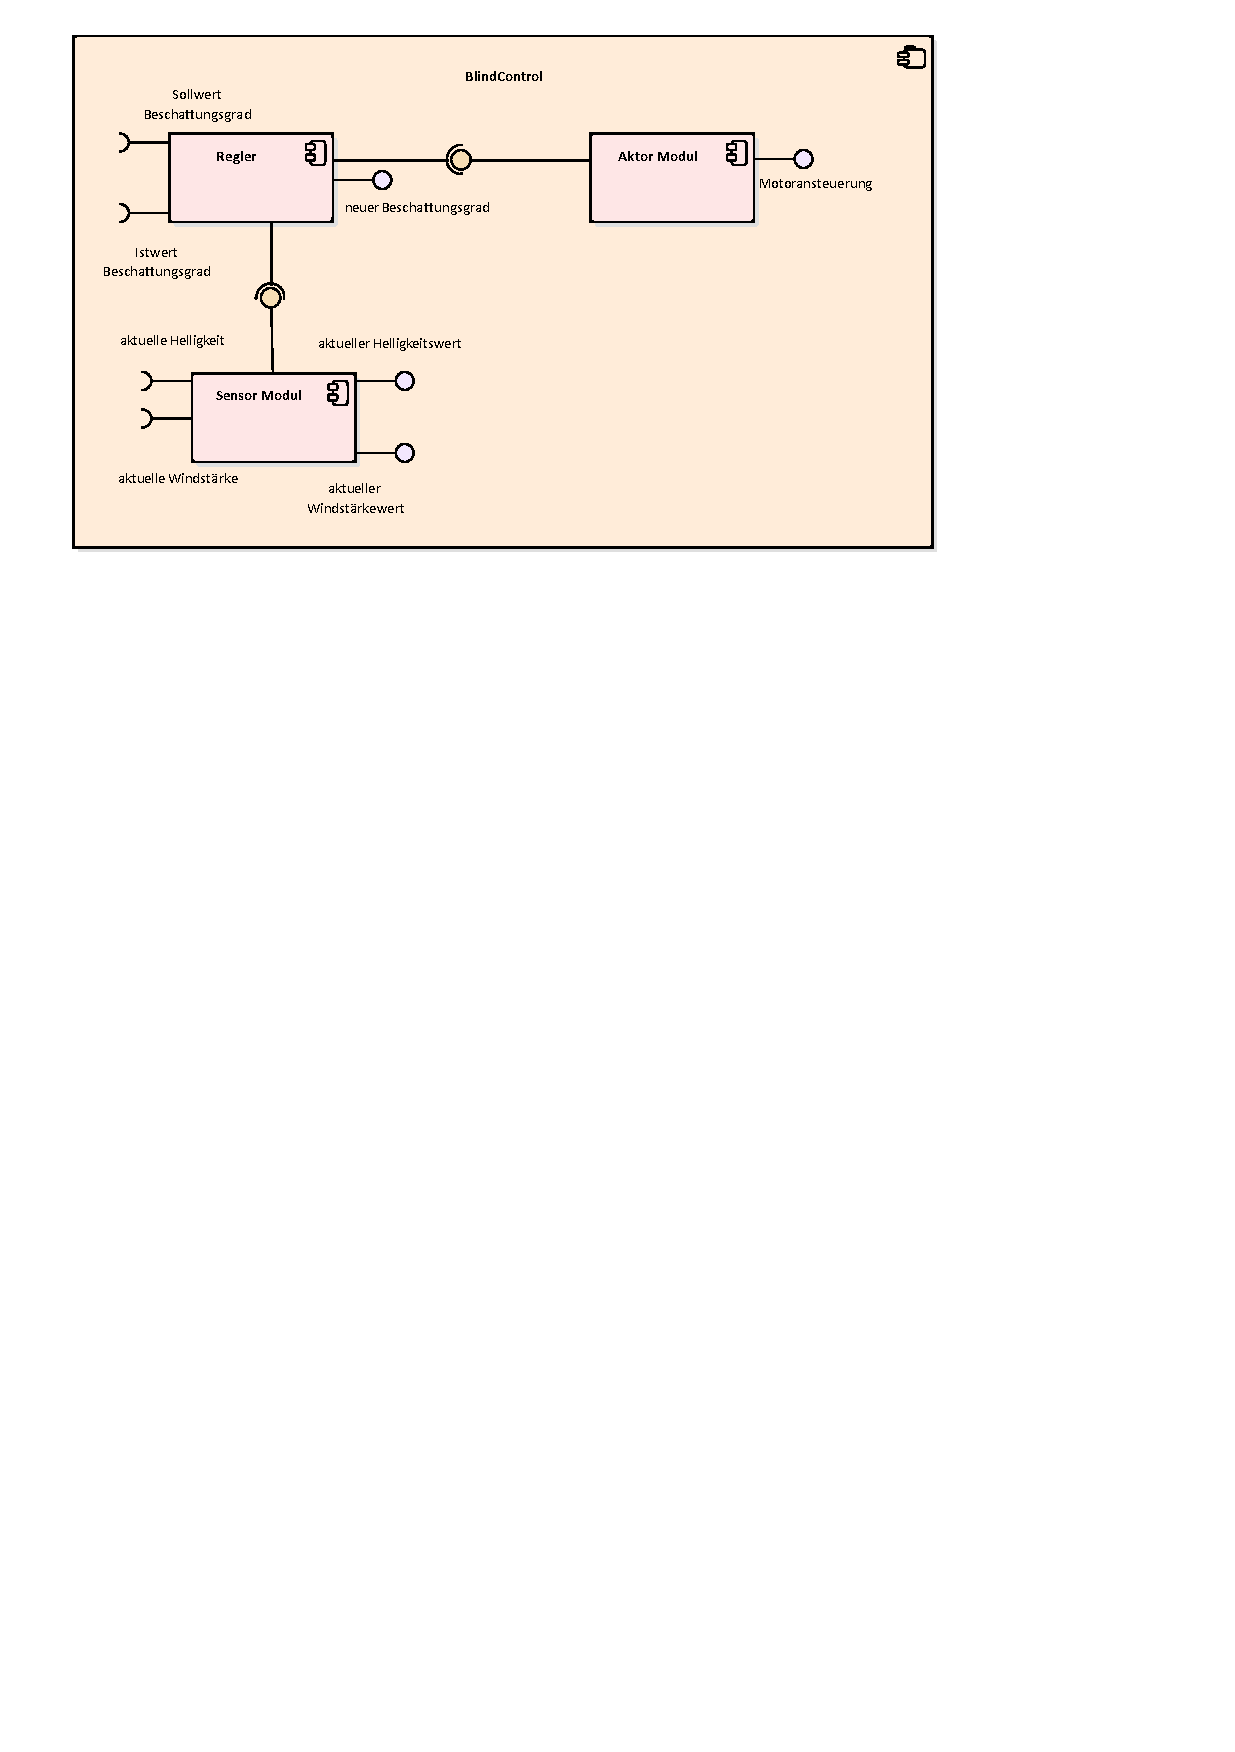
\includegraphics[width=0.7\linewidth]{images/Component}
	\caption[Component Diagramm]{Component Diagramm aller verwendeter Komponenten des Systems.}
	\label{fig:component_diagramm}
\end{figure}

\section{Verhalten}
% mit state or Activity Diagram
Die Abbildung~\ref{fig:Sequence_UseCase} zeigt die Kommunikation zwischen den einzelnen Modulen mit Hilfe von MQTTS, wobei die Darstellung der Kommunikation hierbei zur besseren Übersicht auf das Minimum reduziert ist. Das Regler Modul dient zur Verwaltung aller Steuerungsinputs. Es kann sich bei diesem Input sowohl um Daten von Sensor Modulen, als auch um eine manuelle Ansteuerung handeln, die beispielsweise über eine Sprachsteuerung erfolgt. Auf Basis dieses Inputs entscheidet es, welche Position die Jalousie anfahren soll. Die Anzahl an Sensor Modulen und Modulen, die eine manuelle Ansteuerung vornehmen, ist hierbei nicht begrenzt. Die anzusteuernde Position wird von dem Regler Modul wieder auf das entsprechende Topic (message identifier) gesendet und kann anschließend von einer beliebigen Anzahl an Aktor Modulen ausgelesen werden.

Da der ESP32 über zwei Kerne verfügt und zudem bereits mit FreeRTOS\nomenclature{RTOS}{Real Time Operating System} ausgeliefert wird und dadurch über einen Scheduler verfügt, bietet sich die Nutzung von Tasks an. Zur Darstellung der Funktionsweise werden daher auch hier Sequenzdiagramme genutzt, die die Kommunikation zwischen den einzelnen Tasks zeigen. Abbildung~\ref{fig:Sequence_UserInput} zeigt die Ansteuerung des Aktormoduls. Bei dem User handelt es sich in diesem Fall um das Regler Modul, welches die neue Position mithilfe von MQTTS verschlüsselt überträgt. Der MQTT Task liest die neue Position aus, prüft ob diese zwischen 0 und 100 Prozent liegt und überschreibt die alte Position in einer Queue der Größe 1. Der Motor Control Task liest diese neue Position aus der Queue aus, steuert den Motor der Jalousie an, um die entsprechende Position zu erreichen und speichert die neue Position anschließend im Flash des ESP32, um diese auch nach einem Neustart wieder abrufen zu können. Dennoch kann nicht ausgeschlossen werden, dass aufgrund eines Fehlers die aktuelle Position nicht mit der gespeicherten Position übereinstimmt. Dies hat zur Folge, dass die Jalousie außerhalb des vorgesehen Bereichs von 0-100 Prozent angesteuert wird und dadurch Schaden nimmt. Um dies zu verhindern macht es Sinn an den Bereichsenden, also bei 0 Prozent und 100 Prozent einen Endstopp einzusetzen.

Abbildung~\ref{fig:SequenceMotorControl} zeigt die Implementierung der Endstopps. Der Interrupt Task wird ausgeführt wenn ein Endstopp erreicht wird. Dieser schreibt die Information, welcher Interrupt getriggert wurde, in eine Queue der Größe 10, so dass auch mehrere Interrupts abgespeichert und dann sequentiell abgearbeitet werden können. Der GPIO\nomenclature{GPIO}{General Purpose Input/Output} Task ist ein Task, der die Interrupts aus der Queue ausliest. Handelt es sich um einen Interrupt von einem Endstopp, stoppt er den Motor Control Task, um so zu verhindern, dass dieser den Motor weiter außerhalb des vorgesehenen Bereichs ansteuert. Anschließend korrigiert er die aktuelle Position der Jalousie und speichert diese wieder im Flash ab. Nach der Korrektur erstellt er den Motor Control Task neu, so dass dieser die Position wieder entsprechend eines neuen Inputs ansteuern kann. Eine weitere Anforderung ist es auch, beim Endkunden auf sicherem Weg Updates auf das Endgerät einspielen zu können. Abbildung~\ref{fig:Sequence_Update} zeigt, wie ein entsprechendes Update erfolgt. Hierbei werden zunächst Updateinformationen von einem Webserver geladen. Diese beinhalten die Information, welche Version der Anwendung am aktuellsten ist und auf welchem Server diese sich befinden. Ist die Version der aktuellsten Version neuer, als die aktuell eingesetzte Version, wird diese heruntergeladen. Der ESP32 startet anschließend mit der neuen Version neu. Scheitert dies, fällt er zurück auf die alte Softwareversion. Zur Absicherung der Verbindung wird hierbei TLS als Verschlüsselungsalgorithmus eingesetzt. Weiterhin ist es nicht möglich einen falschen Updateserver anzugeben, da dieser lokal auf dem Gerät hinterlegt ist und durch Secure Boot in Verbindung mit Flash Encryption kann auch ein lokales Einspielen anderer Software, sowie das Auslesen von Informationen wie WLAN Passwörtern, wirkungsvoll verhindert werden. Damit bleibt nur die Möglichkeit, die Updateinformationen direkt auf dem Server zu manipulieren. Standardmäßig werden OTA Updates\nomenclature{OTA Update}{Over The Air Update} mit MD5\nomenclature{MD5}{Message-Digest Algorithm 5} gehasht, was nicht mehr als sicher gilt. Für eine Endanwendung wäre es daher sinnvoll stattdessen beispielsweise sha256\nomenclature{SHA256}{Secure Hash Algorithm 256} zu nutzen. Die vorliegende Implementierung macht hiervon aktuell jedoch keinen Gebrauch. Weiterhin ist die Sicherheit durch die genannten Sicherheitsvorkehrungen bereits bedeutend höher als bei dem Großteil der IoT\nomenclature{IoT}{Internet of Things} Geräte die aktuell zum Einsatz kommen.

Bei der Implementierung des Sensor Moduls besteht insbesondere die Herausforderung einen möglichst geringen Stromverbrauch zu erzielen, um so einen Batteriebetrieb zu ermöglichen. Erreicht werden kann dies durch die Nutzung des Ultra Low Power (ULP)\nomenclature{ULP}{Ultra Low Power} coprocessor des ESP32. Dieser ermöglicht es den ADC\nomenclature{ADC}{Analog-to-Digital Converter} auszulesen, während sich der Hauptprozessor im deep sleep mode befindet. Dieser weckt den Hauptprozessor nur auf wenn die Sensorwerte über die gesetzten Grenzwerte steigt. Bei Sensorwerten wie der Helligkeit die über längere Zeit relativ unverändert bleiben, genügt es hier oft wenn der Hauptprozessor nur ca. einmal pro Strunde aufgerufen wird.Die Tasks für MQTTS und OTA Updates können weitestgehend aus der Implementierung des Aktor Modules übernommen werden. Die Einzige Änderung ist hierbei, dass der MQTT Task die Sensor Daten senden muss, anstatt die Position zu empfangen.

\begin{figure}[hbt]
	\centering
	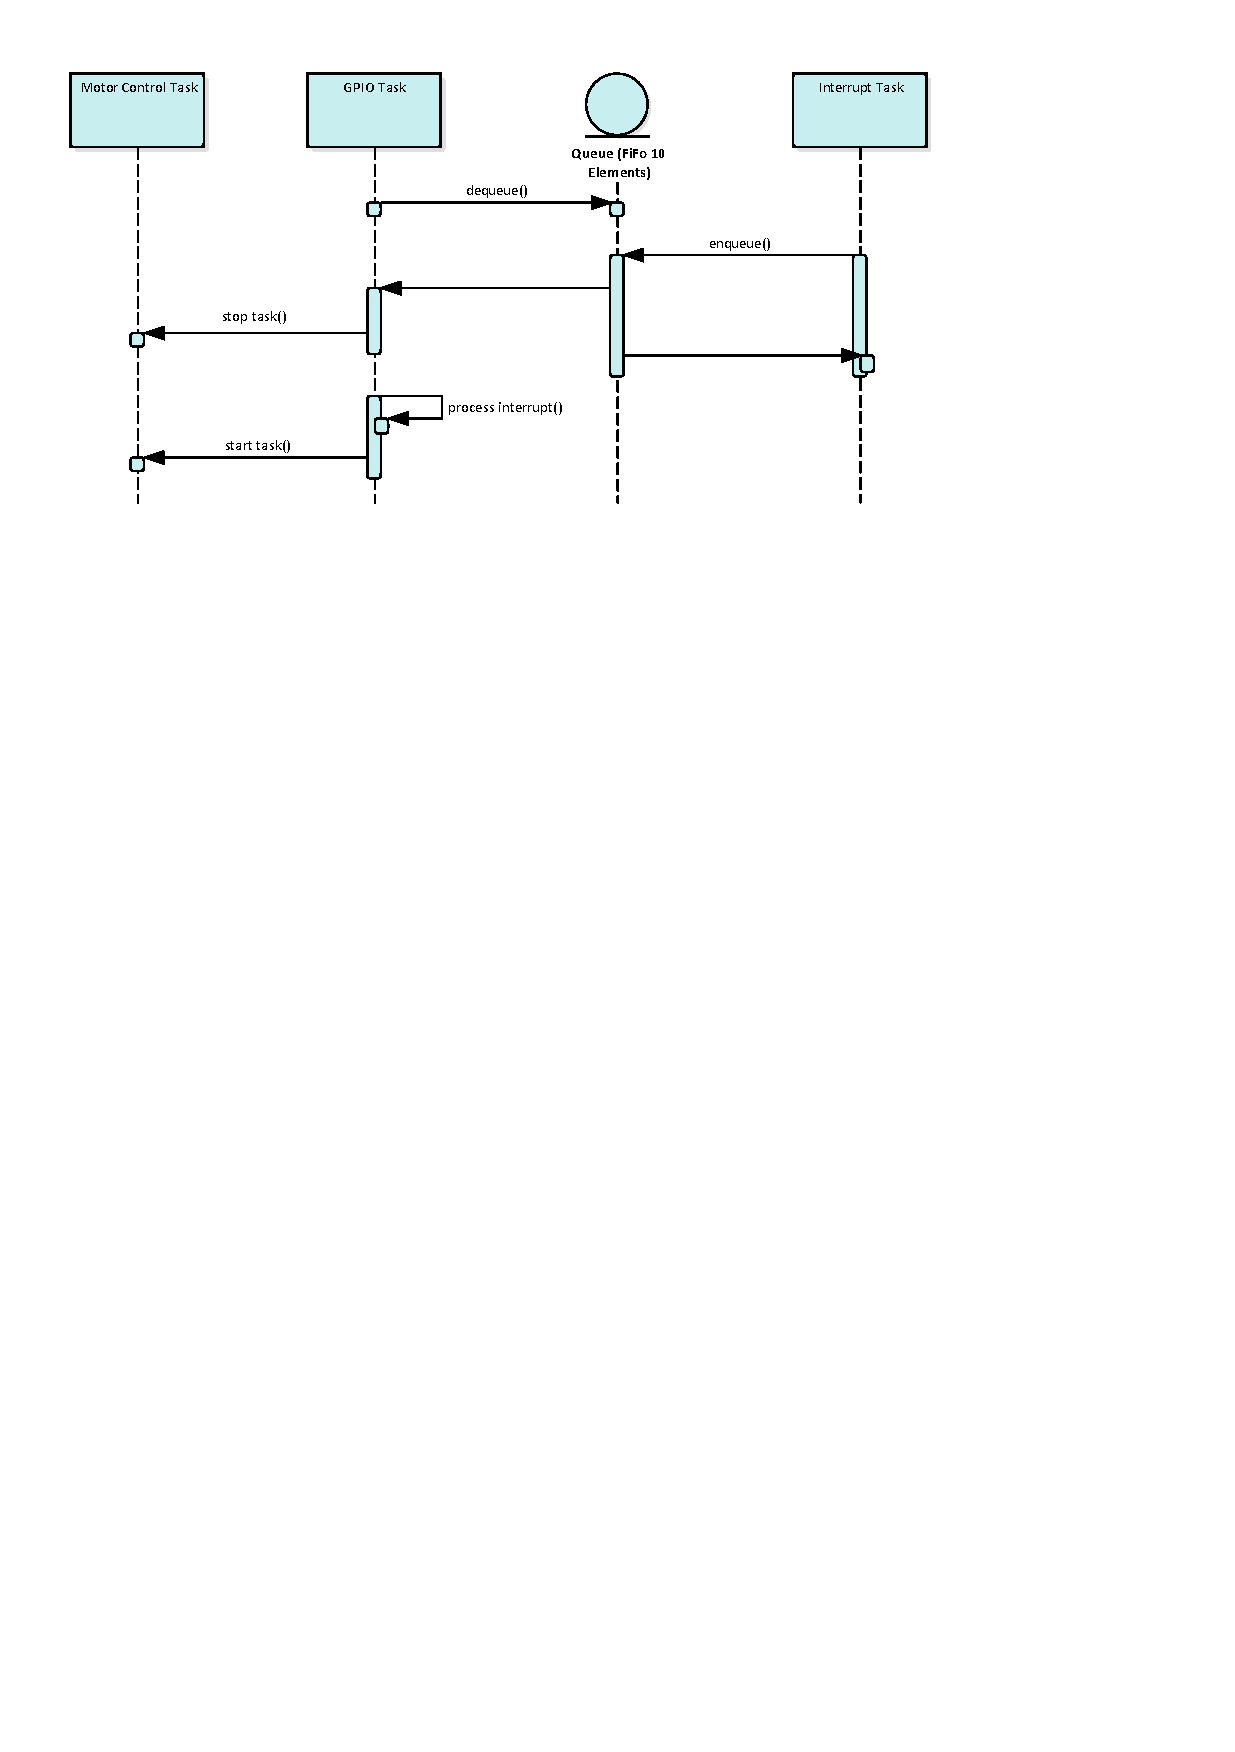
\includegraphics[width=1\linewidth]{images/Sequence_MotorControl}
	\caption[Sequence Diagramm MotorControl]{Sequenz Diagramm der Motorsteuerung.}
	\label{fig:SequenceMotorControl}
\end{figure}

\begin{figure}[hbt]
	\centering
	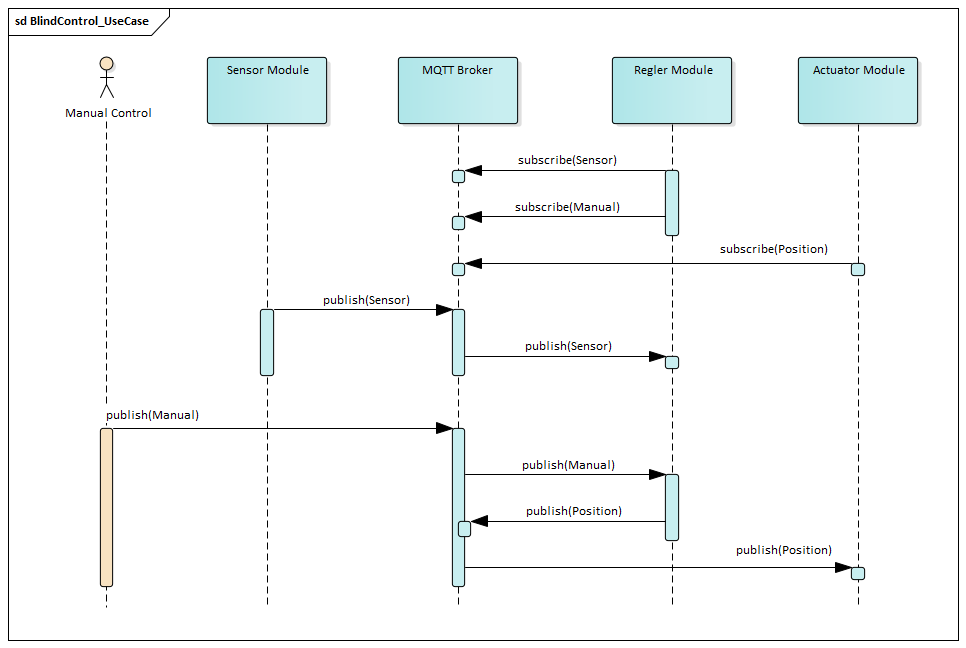
\includegraphics[width=1\linewidth]{images/Sequence_UseCase}
	\caption[Sequence UseCase]{Sequenz Diagramm für die Kommunikation zwischen den einzelnen Modulen.}
	\label{fig:Sequence_UseCase}
\end{figure}

\begin{figure}[hbt]
	\centering
	\includegraphics[width=1\linewidth]{images/Sequence_UserInput}
	\caption[Sequence UserInput]{Sequenz Diagramm für die Ansteuerung des Aktormoduls.}
	\label{fig:Sequence_UserInput}
\end{figure}



\begin{figure}[hbt]
	\centering
	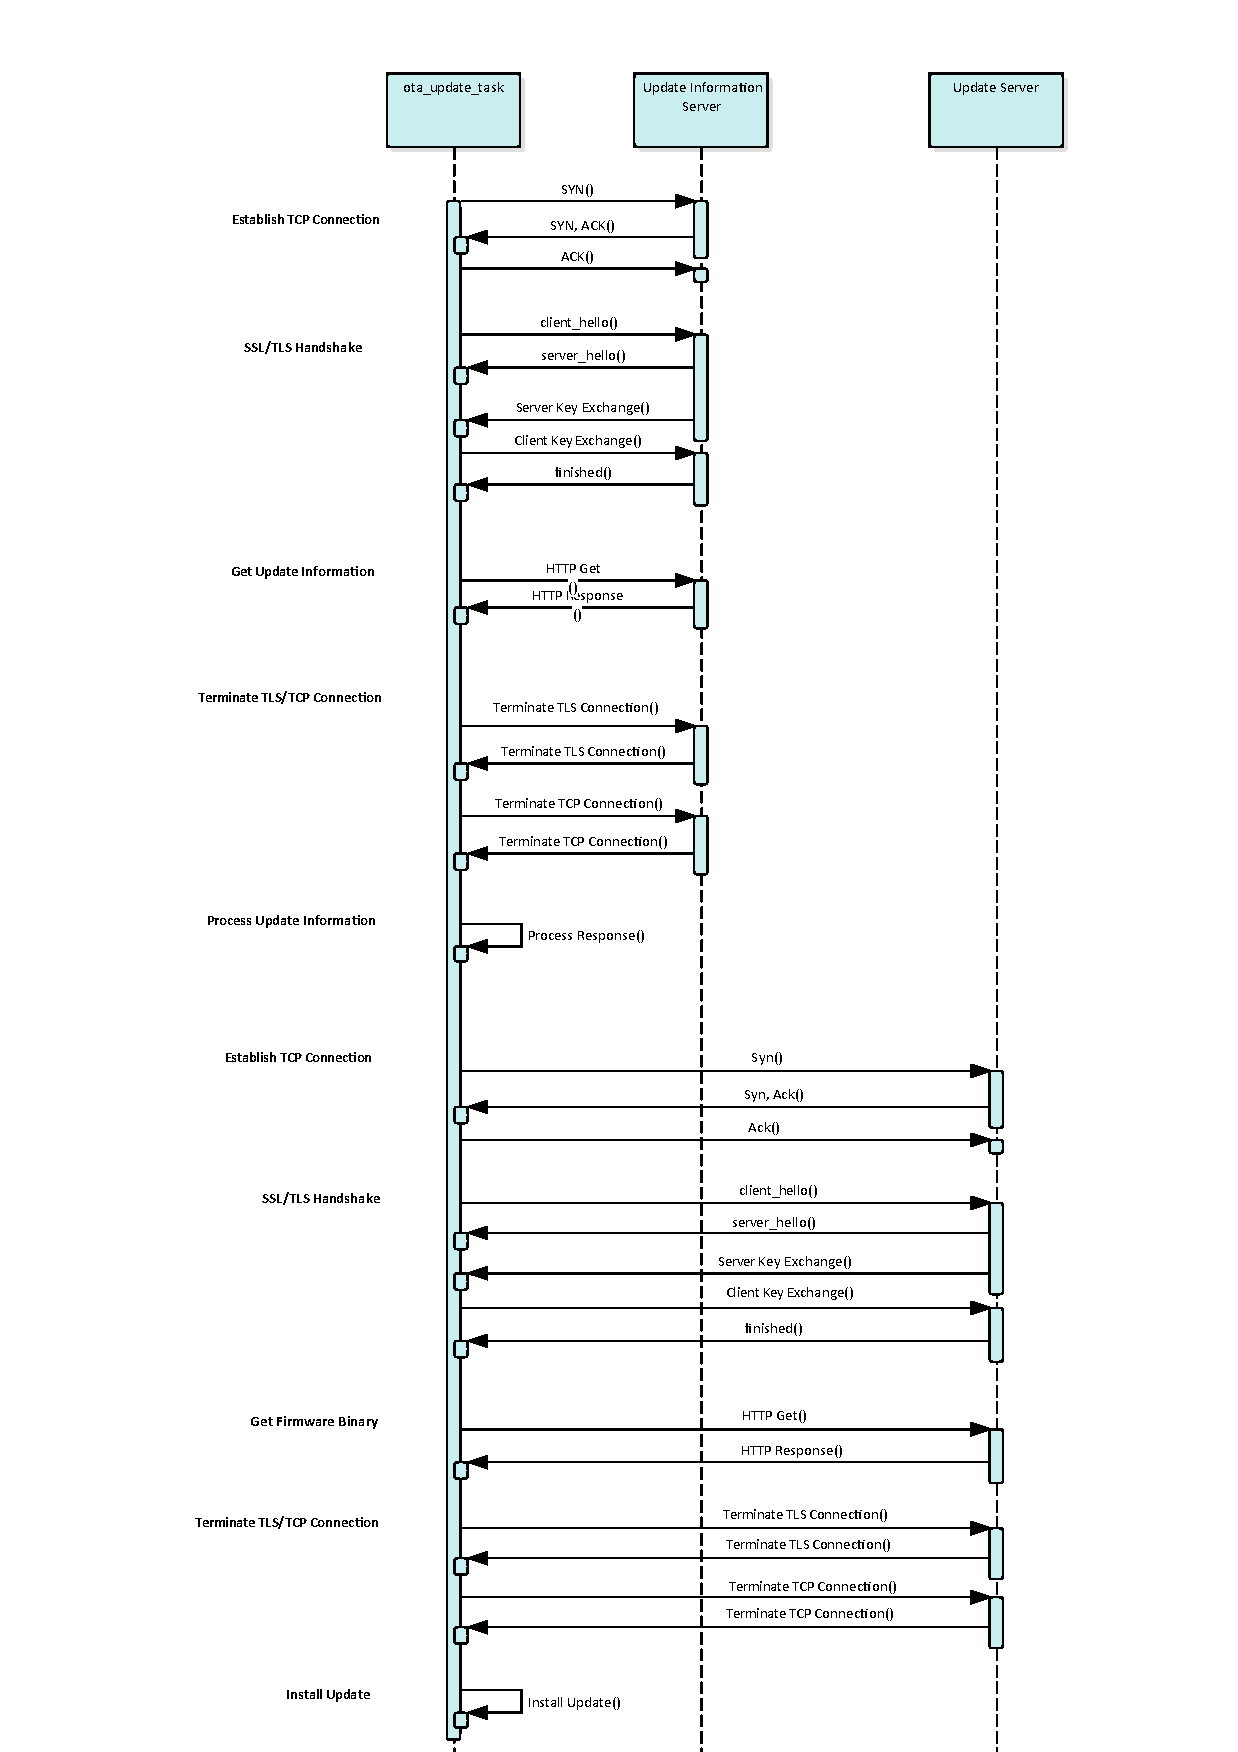
\includegraphics[width=0.7\linewidth]{images/Sequence_Update}
	\caption[Sequence Update]{Sequenz Diagramm zum Ablauf eines Updates.}
	\label{fig:Sequence_Update}
\end{figure}
